\section{目的}
依據 Lab 5（PDF 21--23 頁）觀察三級 CMOS 中第二級的 Miller 耦合，量化過衝、欠衝及負載的影響。

\section{Spec 對照}
\begin{longtable}{p{0.31\linewidth}p{0.29\linewidth}p{0.31\linewidth}}
\toprule
講義要求（PDF頁） & 實作 & 驗證與界線 \\\midrule
步驟 1：三個反相器，觀察第二級突波（21--23） & 01\_miller，case 0 & 已模擬，原生寄生電容保留 \\
步驟 2：加入並改變 $C_c$（22--23） & case 1--3：2/5/10 fF & 含講義 5 fF，已量峰值 \\
問題：加大輸出負載（23） & case 4--5：加 10/40 fF & 固定 $C_c=5$ fF 比較 \\
\bottomrule
\end{longtable}


\section{電路與設計推導}
三個反相器皆採 $W_n/W_p/L=0.6/1.8/0.25\,\mu$m。$C_c$ 接在第二級輸入與輸出之間；第三級始終保留為閘極負載，額外 $C_L$ 接至地。近似耦合關係為 $\Delta V_o\approx C_c\Delta V_i/(C_c+C_{\rm out})$，僅供解釋，實際值由非線性 MOS 模型決定。原始分散的電容案例改為可比對的參數案例，並補上原始程式缺少的尖峰與邊緣量測。

\section{模擬設定}
本次為使用另行提供模型的教學改寫，電源為 1.0 V、溫度為 $25\,^{\circ}\mathrm C$。保留講義指定的拓樸、負載及比較尺寸；原講義的 2.5 V 製程結果不是本次模型的驗收數值。1 V 僅是模擬條件，不能視為模型的安全額定。所有 MOS 的 Bulk 明確接至相應電源軌。

HSPICE S-2021.09 使用 RUNLVL=6；保存波形、列印資料及原生量測。圖表由本次數據重繪；CSV 保存於各 Lab 的 results。完成模擬表示求解成功，並不代表製程可靠度已驗證。加密模型仍有被抑制的警告；既有診斷未取得可判讀的進一步內容，因此不宣稱警告無害或全部模型限制已滿足。

輸入邊緣 0.1 ns，延遲 1 ns、高電位寬度 2 ns、週期 5 ns；暫態 10 ns、列印步距 1 ps。峰值量測窗 0.8--5 ns，rise/fall 定義為 10--90\%／90--10\%。

\section{結果與規格檢查}
六個案例皆正常結束，無 error 或失敗量測。$C_L$ 是第三級閘極負載之外的額外電容。
\begin{center}\small
\begin{tabular}{llllll}
\toprule
$C_c$ (fF) & $C_L$ (fF) & Over (mV) & Under (mV) & $t_r$ (ps) & $t_f$ (ps) \\
\midrule
0 & 0 & 123.09 & 83.47 & 133.70 & 76.70 \\
2 & 0 & 154.03 & 130.47 & 155.08 & 99.82 \\
5 & 0 & 188.80 & 182.72 & 189.49 & 133.95 \\
10 & 0 & 227.81 & 237.61 & 250.08 & 190.65 \\
5 & 10 & 143.98 & 142.61 & 279.78 & 178.15 \\
5 & 40 & 80.57 & 80.85 & 558.95 & 318.36 \\
\bottomrule
\end{tabular}
\end{center}

\begin{figure}[htbp]
\centering
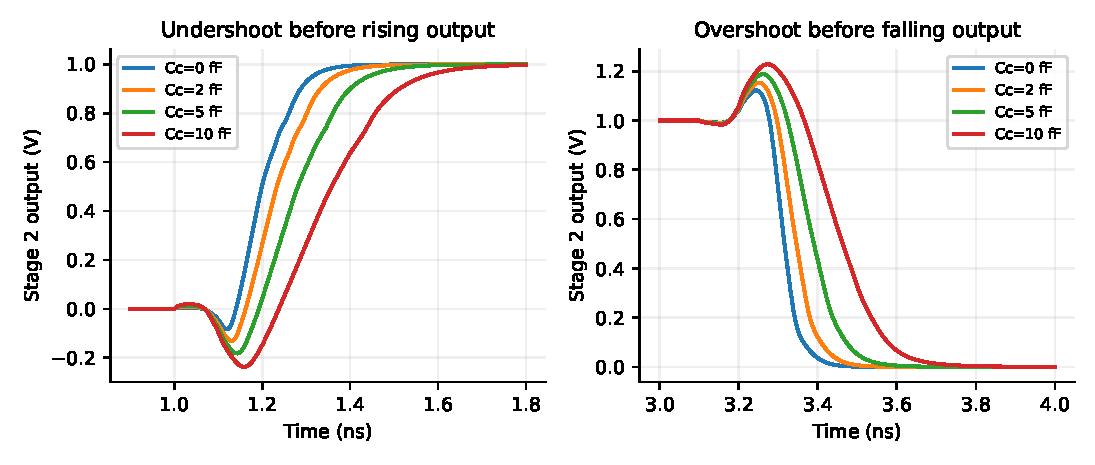
\includegraphics[width=\linewidth]{figures/miller_waveforms.pdf}
\caption{第二級輸出的轉換與尖峰；由本次 HSPICE 數據重繪。}
\end{figure}

\begin{figure}[htbp]
\centering
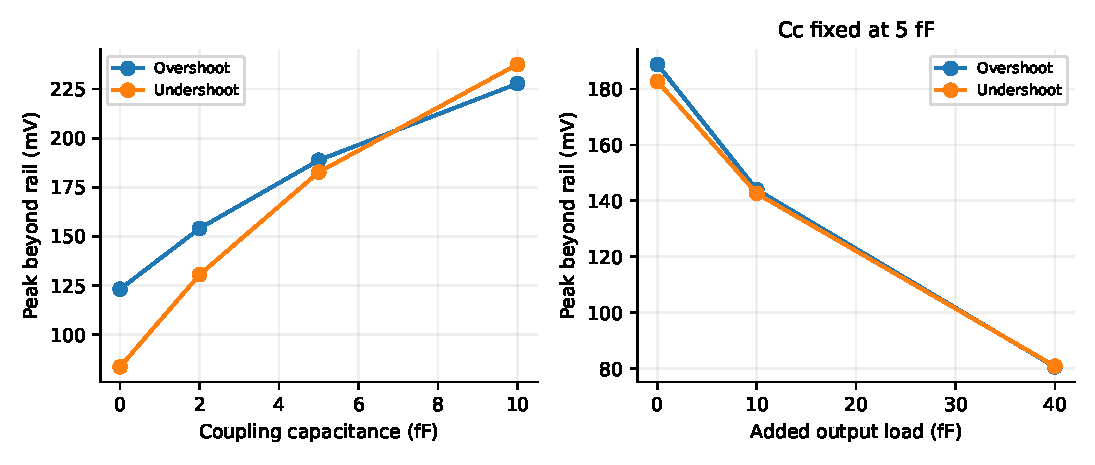
\includegraphics[width=\linewidth]{figures/miller_load_comparison.pdf}
\caption{耦合電容及額外輸出負載的比較；由本次 HSPICE 數據重繪。}
\end{figure}


\section{討論}
當 $C_c$ 從 0 增至 10 fF，過衝由 123.09 增為 227.81 mV，欠衝由 83.47 增為 237.61 mV。固定耦合 5 fF，增加 40 fF 負載使尖峰降至約 80.6/80.9 mV，代價是 rise/fall 增為 559/318 ps。原生模型本身即含耦合，因此 $C_c=0$ 不表示沒有 Miller 效應。尖峰超出電源軌是本次數值結果，不能由此推論硬體可靠度或所有接收端都不受影響。

\section{結論}
兩個實驗步驟與負載問題皆已以實際數據覆蓋；結果支持電容耦合與負載分壓的解釋，適用範圍限於所列模型與刺激。
